\chapter{Numerical model} \label{chap:discretization} %discretized equations?
In this Chapter we describe the methods that are used to discretize the model. 
For the spatial discretization we use the finite volumes methods, which allow 
to solve efficiently flow problems guaranteeing the mass conservation. See 
\cite{fv:leveque} for a broad description.
In the free-flow region we discretize the equations using the staggered grid 
concept, while in the porous-medium we use a cell-centred framework with a Two 
Point Flux Approximation (TPFA).

For the temporal discretization we use implicit finite differences methods, 
like Backward Euler (BE) and the Backward Differencing Formula 2 (BDF2).
%
\section{Staggered grid concept}
The staggered grid concept is characterized by the distinction between the 
degrees of freedom related to scalar primary variables and those related to 
vectorial primary variables. It is useful for the discretization through finite 
volumes of saddle point problems, like the Navier-Stokes or RANS equations. 
Indeed, in these kind of problems, if we locate all the primary variables, i.e. 
pressure, velocity and possibly the turbulent kinetic energy and its 
dissipation rate, at the same positions in the grid, spurious mode in the 
solution may arise, leading to wrong results. A possible fix to this issue 
is thus to store the primary variables in a \emph{staggered} fashion, putting 
the degrees of freedom related to scalar variables at the centre of the cells 
and those related to vectorial variables on the faces, aligned to the faces 
normal direction. Therefore we obtain different control volumes for the 
variables, as we can see in Figure~\ref{fig:staggrid} for the case of the 
Navier-Stokes equations in a two-dimensional domain.
\begin{figure}[t]
	\centering
%	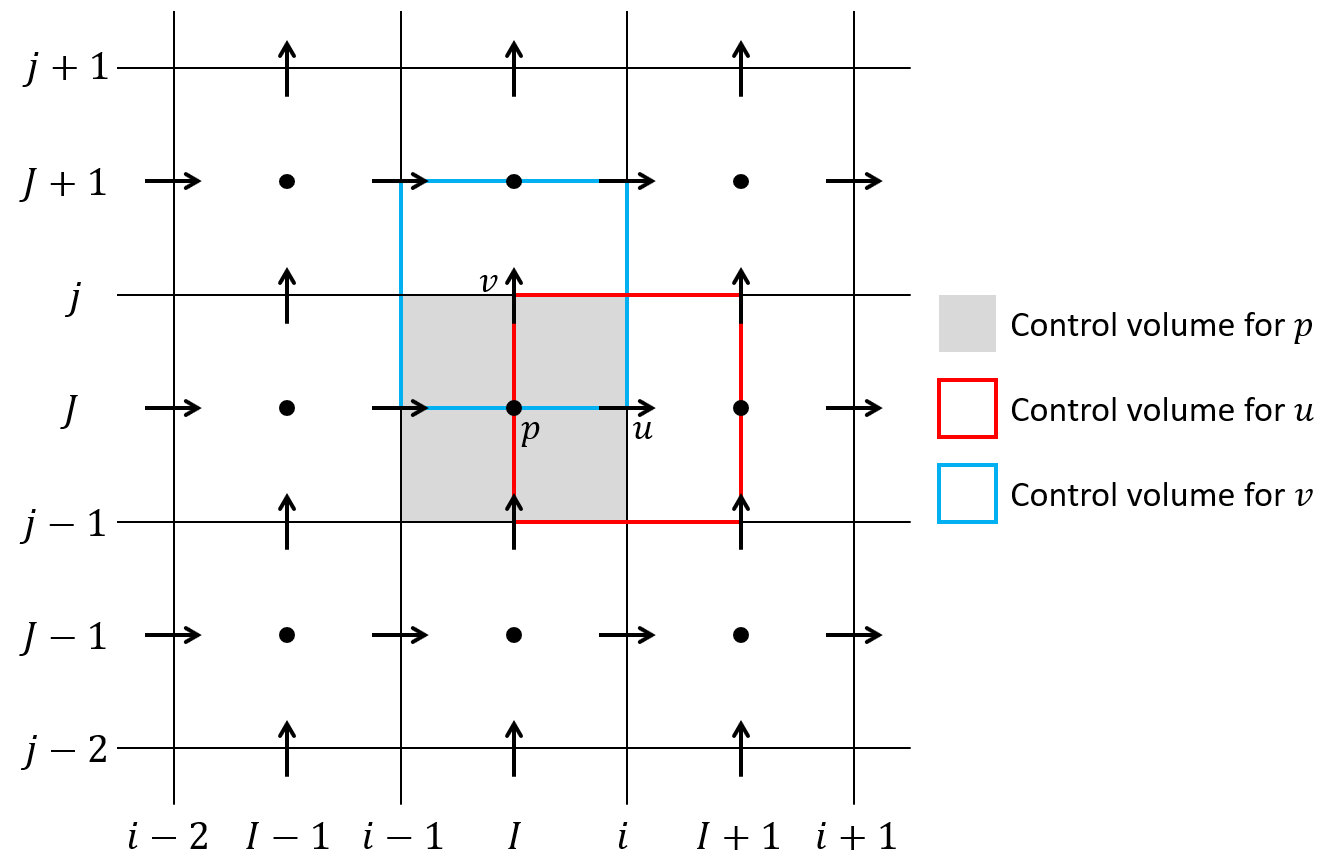
\includegraphics[width=\textwidth]{staggered_grid_mia_ij.png}
	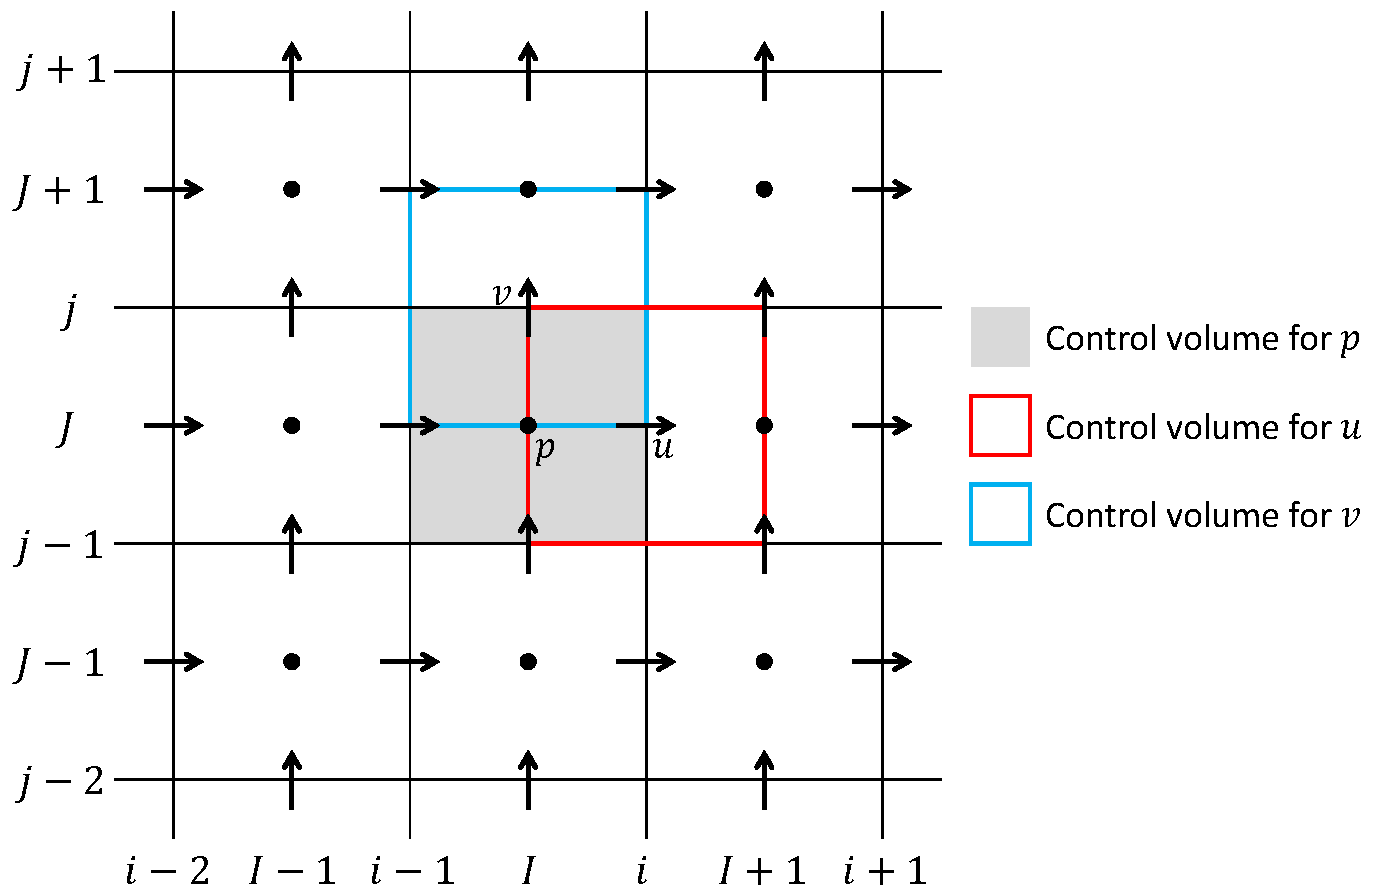
\includegraphics[width=\textwidth]{staggered_grid_mia.pdf}
	\caption[Staggered grid control volumes]{An example of a staggered grid 
	with the pressure degrees of freedom (dofs) stored at the centres of the 
	cells and the velocity dofs stored on the faces. The different control 
	volumes are highlighted. The indices in capital letters $\dots,I,I+1,\dots$ 
	and $\dots,J,J+1,\dots$ refer to cells, thus to the position of 
	cell-centred variables, while the indices in lower case letters 
	$\dots,i,i+1,\dots$ and $\dots,j,j+1,\dots$ refer to faces, thus to the 
	position of staggered variables.}
	\label{fig:staggrid}
\end{figure}

This approach is known also as Marker and Cell (MAC), as it was called in its 
first appearance in a paper by \textcite{stagg:orig}, within a finite 
differences framework. A more recent description can be found in 
\cite{main:vermal}.

Another advantage of this discretization method is that on the boundary we have 
the degrees of freedom of the normal component of the velocity, so it is easier 
to impose boundary and interface conditions.

For the sake of simplicity we consider now a bi-dimensional domain and 
$\mathbf{v} = [u, v]^{\mathrm{T}}$.
%
\subsection{Cell-centred equations}
\subsubsection{Continuity equation}
The continuity equation \eqref{eq:ransmass} can be discretized straight forward 
because it does not involve the density. We integrate over the ``grey'' control 
volume $V_p = [i-1,i] \times [j-1,j]$, according to Figure~\ref{fig:staggrid}, 
and we apply the Gauss's divergence theorem:
\begin{equation}
\int_{V_p} \nabla \cdot \mathbf{v} \; dV = \int_{\partial V_p} \mathbf{v} \cdot 
\mathbf{n} \; dA = 0.
\end{equation}
The integral over the boundary $\partial V_p$ can be split over the four edges, 
that we identify with $e_p$ (east), $n_p$ (north), $w_p$ (west), $s_p$ (south):
\begin{equation}
\int_{\partial V_p} \mathbf{v} \cdot \mathbf{n} \; dA = \int_{e_p} u \; dA
+ \int_{n_p} v \; dA - \int_{w_p} u \; dA - \int_{s_p} v \; dA.
\end{equation}
At this point we discretize the equation approximating the values of the 
velocity with the value at the centre of the edges, for example:
\begin{equation}
\int_{e_p} u \; dA \simeq u_{i,J} |{e_p}|,
\end{equation}
thus obtaining
\begin{equation}
	u_{i,J} |e_p| + v_{I,j}|n_p| - u_{i-1,J}|w_p| - v_{I,j-1}|s_p| = 0
\end{equation}
\subsubsection{Turbulence model equations}
The equations for the turbulent kinetic energy \eqref{eq:komegak} and the 
specific dissipation rate $\omega$ are treated analogously to the continuity 
equation, but they involve more terms.
\subsection{Staggered equations}
The momentum equation \eqref{eq:ransmom2} is discretized using the staggered 
control volumes. Let us consider the equation for the component $u$:
\begin{equation}
\frac{\partial{(\varrho u)}}{\partial t} + \nabla \cdot (\varrho u 
\mathbf{v}) - \nabla \cdot (\mu_\text{eff} \nabla u) + 
\frac{\partial}{\partial x} \big(p + \varrho k\big) = 0.
\end{equation}
Notice that, since we are considering a two-dimensional model, we have 
substituted the factor $2/3$ with a $1$ in front of $\varrho k$, because it 
came from the requirement \eqref{eq:tracciatau}.

We integrate it over the ``red'' control volume $V_u=[I, I+1]\times[j-1,j]$, 
according to Figure~\ref{fig:staggrid}, and apply the Gauss's divergence 
theorem:
\begin{multline} \label{eq:stagmomeq}
\int_{V_u} \bigg[ \frac{\partial{(\varrho u})}{\partial t} + \nabla 
\cdot (\varrho u \mathbf{v} ) - \nabla \cdot (\mu_\text{eff} \nabla u) + 
\frac{\partial}{\partial x}\big( p + \varrho k \big) \bigg ]\; dV 
=\\
=\frac{d}{dt} \int_{V_u} \varrho u\; dV + \int_{\partial V_u} \varrho u 
(\mathbf{v} \cdot \mathbf{n}) \; dA -\\
- \int_{\partial V_u} \mu_\text{eff} 
(\nabla u \cdot \mathbf{n}) \; dA + \int_{\partial V_u} (p + \varrho k) n_x \; 
dA = 0,
\end{multline}
where $n_x$ is the component in the $x$ direction of the outward unit 
normal $\mathbf{n}$. Let us identify again the four edges of $\partial V_u$ 
with $e_u$ (east), $n_u$ (north), $w_u$ (west), $s_u$ (south), so that
\begin{equation}
	\partial V_u = e_u \cap n_u \cap w_u \cap s_u.
\end{equation}
In the equation \eqref{eq:stagmomeq} there are four terms of different kinds, 
let us consider each of them separately, starting from the simplest one:
\begin{itemize}
	\item in the storage term we approximate the velocity with the value at the 
	centre of the control volume:
	\begin{equation}
	\frac{d}{dt} \int_{V_u} \varrho u\; dV \simeq \frac{d}{dt} \big( \varrho 
	u_{i,J} \big)|V_u|;
	\end{equation}
	%
	\item in the pressure term the contributions from the edges $n_u$ and $s_u$ 
	is null because $n_x=0$ on them, so 
	\begin{equation}
	\int_{\partial V_u} (p + \varrho k)n_x \; dA = \int_{e_u} (p+\varrho k) \; 
	dA - \int_{w_u} (p+\varrho k) \; dA.
	\end{equation}
	Then we approximate $p$ and $k$ with the values at the centre of the edges:
	\begin{equation}
	\int_{e_u} (p+\varrho k) \; dA \simeq (p_{I+1,J} +\varrho k_{I+1,J}) |e_u|,
	\end{equation}
	\begin{equation}
	\int_{w_u} (p+\varrho k) \; dA \simeq (p_{I,J} +\varrho k_{I,J}) |w_u|.
	\end{equation}
	%
	\item in the diffusive term we have both a frontal momentum flux 
	contribution from the edges $e_u$ and $w_u$ and a lateral momentum flux 
	contribution from the edges $n_u$ and $s_u$:
	\begin{multline}
	\int_{\partial V_u} \mu_\text{eff} (\nabla u \cdot \mathbf{n}) \; dA =     
	\int_{e_u} \mu_\text{eff} \frac{\partial u}{\partial x} \; dA
	- \int_{w_u} \mu_\text{eff} \frac{\partial u}{\partial x} \; dA \;+\\
	+\int_{n_u} \mu_\text{eff} \frac{\partial u}{\partial y} \; dA
	- \int_{s_u} \mu_\text{eff} \frac{\partial u}{\partial y} \; dA
	\end{multline}
	We develop the contributions from $e_u$ and $n_u$, the other two are 
	analogous.\\	
	For the frontal momentum flux we approximate the viscosity with 
	the value at the centre of the edge, while we approximate the derivative of 
	the velocity with a centred finite difference:
	\begin{equation}
	\int_{e_u} \mu_\text{eff} \frac{\partial u}{\partial x} \; dA \simeq 
	\mu_{\text{eff},\{I+1,J\}} \frac{u_{i+1,J} - u_{i,J}}{\Delta x} |e_u|,
	\end{equation}
	where $\Delta x$ is the distance between the coordinate of $i$ and the one 
	of $i+1$ along the $x$-axis. For the lateral momentum flux we split the 
	edge $n_u$ into the two halves related to the two cells 
	$[i-1,i]\times[j-1,j]$ and $[i,i+1]\times[j-1,j]$:
	\begin{equation}
	n_u = [I,i]\times \{j\} \cup [i,I+1] \times \{j\}.
	\end{equation}
	We employ again a centred finite difference to approximate of the 
	derivative of the velocity, while, for the approximation of the viscosity, 
	we compute an average between the two cells sharing the face:
	\begin{equation}
	\int_{n_u} \mu_\text{eff} \frac{\partial u}{\partial y} \; dA = 
	\int_{\{I,j\}}^{\{i,j\}} \mu_\text{eff} \frac{\partial u}{\partial y} \; dA 
	+\int_{\{i,j\}}^{\{I+1,j\}} \mu_\text{eff} \frac{\partial u}{\partial y} \; 
	dA
	\end{equation}
	\begin{equation*}
	\int_{\{I,j\}}^{\{i,j\}} \mu_\text{eff} \frac{\partial u}{\partial y} \; dA 
	\simeq \frac{1}{2}\big(\mu_{\text{eff},\{I,J\}}+\mu_{\text{eff},\{I,J+1\}} 
	\big) \frac{u_{i,J+1}-u_{i,J}}{\Delta y} \frac{|n|}{2} 
	\end{equation*}
	\begin{equation*}
	\int_{\{i,j\}}^{\{I+1,j\}} \mu_\text{eff} \frac{\partial u}{\partial y} \; 
	dA \simeq \frac{1}{2}\big( \mu_{\text{eff},\{I+1,J\}}+ 
	\mu_{\text{eff},\{I+1,J+1\}} \big) \frac{u_{i,J+1}-u_{i,J}}{\Delta y} 
	\frac{|n|}{2},
	\end{equation*}
	where $\Delta y$ is the distance between the coordinate of $J$ and the one 
	of $J+1$ along the $y$-axis.
	%
	\item in the convective term we have again both a frontal momentum flux 
	contribution from the edges $e_u$ and $w_u$ and a lateral momentum flux 
	contribution from the edges $n_u$ and $s_u$:
	\begin{multline}
	\int_{\partial V_u} \varrho u (\mathbf{v} \cdot \mathbf{n}) \; dA = 
	\int_{e_u} \varrho u u \; dA - \int_{w_u} \varrho u u \; dA \; +\\
	+ \int_{n_u} \varrho u v \; dA  -\int_{s_u} \varrho u v \; dA.
	\end{multline}
	For the discretization we have to distinguish between the 
	\emph{transporting} velocity, coming from $\mathbf{v} \cdot \mathbf{n}$, 
	and the \emph{transported} field, coming from $\varrho u$, that in this 
	case of incompressible flow is only the velocity because the density is 
	constant. For the former we average between the values sharing the edge, 
	while for the latter we have to consider an approximation that takes into 
	account the flow direction, as it will be explained in detail in 
	Subsections~\ref{subsec:diffscheme} and \ref{subsec:tvd}. For the moment we 
	simply denote this approximation with a superscript $^*$.
	We develop only the contributions from $e_u$ and $n_u$, the other two are 
	analogous.\\
	For the frontal momentum flux we approximate the transporting velocity with 
	an average between the values of the two staggered cells sharing the 
	staggered edge:
	\begin{equation}
		\int_{e_u} \varrho u u \; dA \simeq \varrho u^* \frac{u_{i,J} + 
		u_{i+1,J}}{2}|e_u|.
	\end{equation}
	For the lateral momentum flux we approximate the transporting velocity with 
	an average between the values a the two ends of the edge:
	\begin{equation}
	\int_{n_u} \varrho u v \; dA \simeq \varrho u^* \frac{v_{I,j} 
	+v_{I+1,j}}{2} |n_u|.
	\end{equation}
	
\end{itemize}

The equation for the component $v$ of the velocity is analogous with the only 
addition of the gravity term:
\begin{equation}
\frac{\partial{(\varrho v)}}{\partial t} + \nabla \cdot (\varrho v 
\mathbf{v}) - \nabla \cdot (\mu_\text{eff} \nabla v) + 
\frac{\partial}{\partial y} \big(p + \varrho k\big) - \varrho g= 0,
\end{equation}
with $g = \SI{-9.81}{m/s}$. The gravity term is discretized straight-forward:
\begin{equation}
\int_{V_v} \varrho g \; dV = \varrho g |V_v|,
\end{equation}
where $V_v = [i-1, i] \times [J, J+1]$ is the ``blue'' control volume in 
Figure~\ref{fig:staggrid}. 

%
\subsection{Differencing schemes} \label{subsec:diffscheme} %Linear 
%differencing schemes ?
How to choose the scheme for the approximation of the transported field?
It holds in general for every equation involving a convective term.
These are easy but sometimes may produce oscillations, they make use of a 
bigger stencil.
\begin{itemize}
\item Centred Differencing (CD) scheme:
\begin{equation} \label{eq:cd}
\phi^* = \frac{\phi^U + \phi^D}{2}
\end{equation}
\item Linear Upwind Differencing (LUD) scheme:
\begin{equation} \label{eq:lud}
\phi^* = \frac{3\phi^U - \phi^{UU}}{2}
\end{equation}
\item Quadratic Upstream Interpolation for Convective Kinetics (QUICK) scheme 
\cite{fv:leonard}:
\begin{equation} \label{eq:quick}
	\phi^* = \frac{3\phi^D + 6 \phi^U - \phi^{UU}}{8}
\end{equation}
\end{itemize}
A complete description can be found for example in \cite{main:vermal}.
\subsection{TVD methods} \label{subsec:tvd}
Total Variation Diminishing (TVD) methods have been developed originally for 
scalar conservation laws of the type:
\begin{align}
	\label{eq:conslaw} &\frac{d\phi}{dt} + \frac{d}{dx}\big(f(\phi)\big) = 0, 
%\quad t>0 \quad x 
%	\in 
%	\mathbb{R}\\[1ex]
%	\label{eq:conslawic} &\phi(x, 0) = \phi_0(x), \quad x \in \mathbb{R}
\end{align}

\begin{defn}
	The \emph{total variation} of the numerical solution of the problem 
	\eqref{eq:conslaw} is defined as:
	\begin{equation}
		TV(\phi) = \sum_{i=1}^{N_\text{dof}-1} |\phi_{i+1} - \phi_i|,
	\end{equation}
	where $i$ represents the index of the nodes of the discretized domain, so 
	it is the sum of the jumps between all the couples of adjacent nodes.
\end{defn}
\begin{defn}
	A method is called \emph{TVD} if the total variation of the solution does 
	not increase with time, i.e. 
	\begin{equation}\label{eq:tvdcondition}
	TV(\phi ^{n+1}) \leq TV(\phi^n) \quad \forall n>0,
	\end{equation}
	where $\phi^n$ is the numerical solution at the time-step $t^n$.
\end{defn}

Their aim of TVD methods is to provide a solution with a second order accuracy 
and without any overshoot or undershoot, these kind of methods are called also 
\emph{high resolution methods}. Starting from this second feature, the 
property 
that we are interested in is monotonicity:
\begin{defn}
	A scheme is called \emph{monotonicity preserving} if it does not create new 
	local extrema, local minima are non-decreasing and local maxima are 
	non-increasing.
\end{defn}
In \cite{tvd:monotonicity} it has been proved that a TVD scheme is 
monotonicity 
preserving, so imposing \eqref{eq:tvdcondition} we should avoid the 
development 
of solutions containing overshoots and undershoots, as it can happen using 
methods like QUICK.

According to \cite{tvd:sweeby} and \cite{main:darwish} we can achieve our 
target adding to the first order upwind approximation a second order 
non-linear 
anti-diffusive flux: 
\begin{equation} \label{eq:tvdformula}
\phi_e = \phi^U + \frac{1}{2}\psi(r)(\phi^D - \phi^U), \quad r = 
\frac{\phi^U - \phi^{UU}}{\phi^D - \phi^U}.
\end{equation}
The flux includes a function $\psi(r)$ called \emph{flux limiter} that should 
dampen the second order contribution in regions where it could produces 
oscillations. It is chosen non-negative in order to preserve the sign of the 
flux and it depends on the variable $r$ that is defined as the ratio between 
two consecutive gradients. The non linearity can not be avoided, indeed it was 
proved by Godunov that any monotonicity preserving linear scheme can be at 
most 
first order accurate (see \cite{tvd:godunov}).

Exploiting the approximation \eqref{eq:tvdformula} to solve the problem 
\eqref{eq:conslaw} and imposing the TVD condition on the solution we obtain 
the 
following bounds for the flux limiter:
\begin{align}
\psi(r) = 0 \quad &\text{if} \quad r < 0\\
\psi(r) \leq \min \{2r, 1\} \quad &\text{if} \quad 0 \leq r \leq 1\\
\psi(r) \leq 2 \quad &\text{if} \quad r > 2
\end{align}
Notice that when $r<0$ we are near to a local maximum or minimum, because it 
means that the difference between the upstream and downstream nodes has the 
opposite sign of that one between the far upstream and upstream nodes. In this 
situation we set $\psi = 0$ i.e. we use the first order upwind.
It is also convenient if $\psi(r)$ has the following symmetry property:
\begin{equation}
\frac{\psi(r)}{r} = \psi\bigg(\frac{1}{r}\bigg)
\end{equation}
which ensures that backward- and forward-facing gradients are treated in the 
same way.

Following \cite{tvd:sweeby} and \cite{tvd:vanleer}, any second order scheme 
can 
be obtained as a convex combination of the CD scheme \eqref{eq:cd} and LUD 
scheme \eqref{eq:lud}, moreover $\psi(r)$ should be at least Lipschitz 
continuous. Thus, adding these requirements to the previous ones, we obtain 
the 
following bounds for the flux limiter function of a TVD method:
\begin{align}
\psi(r) = 0 \quad &\text{if} \quad r < 0 \notag \\
\label{tvd:bounds} r \leq \psi(r) \leq \min \{2r, 1\} \quad &\text{if} \quad 0 
\leq r \leq 1\\
1 \leq \psi(r) \leq \min \{r, 2 \} \quad &\text{if} \quad r > 2 \notag
\end{align}
% A livello teorico potrei aggiungese la dimostrazione di monotonicity->TVD, 
%l'applicazione di TVD per ottenere i bounds e l'applicazione dei bounds 
%all'approssimazione col flux limiter (come in sweby o in darwish). Potrei 
%mettere qualcosa nell'appendice.
\subsubsection{Flux limters}
Starting from the bounds \eqref{tvd:bounds} it is easy to create a 
flux limiter function, indeed in literature many possible choices can be 
found. 
We list here some of the most popular functions that have been implemented in 
\DUMUX and in Figure~\ref{fig:fluxlimiters} we can see their graph in the 
Sweby's diagram:
\begin{itemize}
	\item Van Leer \cite{tvd:vanleer}
	\begin{equation} \label{eq:vl}
	\psi(r) = \frac{r+|r|}{1+r}.
	\end{equation}
	It is a smooth function that asymptotically reaches 2 for $r \rightarrow 
	\infty$.
%
	\item Van Alabada \cite{tvd:vanalabada}
	\begin{equation}
	\psi(r)=
	\begin{cases}
	\dfrac{r^2+r}{r^2+1} \quad &\text{if $r\geq 0$}\\[2ex]
	0 \quad &\text{if $r<0$}
	\end{cases}
	\end{equation}
	It is a smooth function that instead goes to 1 as $r \rightarrow \infty$.
%
	\item Min-Mod \cite{tvd:roe}
	\begin{equation}
	\psi(r) = \max \{0, \min \{ r,1\} \}
	\end{equation}
	It is a piecewise linear function that stays on the lower boundary of the 
	TVD region. Using this limiter we add to the upwind value an increment 
	equal to the smallest variation between $\phi^{UU}-\phi^U$ and $\phi^D - 
	\phi^U$.
%
	\item Superbee \cite{tvd:roe}
	\begin{equation}
	\psi(r)=\max \{0, \min \{ 2r, 1\}, \min \{ r, 2\} \}
	\end{equation}
	It is a piecewise linear function that stays on the upper boundary of the 
	TVD region.
%
	\item UMIST \cite{tvd:lien}
	\begin{equation}
	\psi(r)=\max \bigg\{0, \min \bigg\{ 2r, \frac{3r+1}{4},\frac{r+3}{4}, 
	2\bigg\} \bigg\}
	\end{equation}
	It is a piecewise linear function that was designed as a symmetrical TVD 
	version of QUICK.
%
	\item MC (Monotinized Central) limiter \cite{tvd:mclimiter}
	\begin{equation}
	\psi(r)=\max \bigg\{0, \min \bigg\{ 2r, \frac{r+1}{2}, 2\bigg\} \bigg\}
	\end{equation}
	It is also known as MUSCL (Monotonic Upstream-Centred Scheme for 
	Conservation Laws) limiter.
%	
%	\item WAHYD \cite{nonunif:hou}
%	\begin{equation}
%	\psi(r)=
%	\begin{cases}
%	\dfrac{r + |r|}{r + 1} & \text{if $r \leq 1$} \\[2ex]
%	\min \bigg\{ \dfrac{r + 2 r^2}{2 + r^2}, 2 \bigg\} & \text{if $r>1$}
%	\end{cases}
%	\end{equation}
%	It is a hybrid scheme, for $r\leq 1$ it is the Van Leer scheme 
%	\eqref{eq:vl}, while for $r>1$ it is closer to the upper bound of the TVD 
%	region.
\end{itemize}

\begin{figure}
	\centering
	% This file was created by matlab2tikz.
%
\definecolor{mycolor1}{rgb}{0.92900,0.69400,0.12500}%
\definecolor{mycolor2}{rgb}{0.49400,0.18400,0.55600}%
\definecolor{mycolor3}{rgb}{0.46600,0.67400,0.18800}%
\definecolor{mycolor4}{rgb}{0.30100,0.74500,0.93300}%
\definecolor{mycolor5}{rgb}{0.63500,0.07800,0.18400}%
\definecolor{mycolor6}{rgb}{0.00000,0.44700,0.74100}%
%
\begin{tikzpicture}

\begin{axis}[%
width=4.521in,
height=3.566in,
at={(0.758in,0.481in)},
scale only axis,
xmin=0,
xmax=5.5,
xlabel={$r$},
ymin=0,
ymax=3,
ylabel style={rotate=-90},
ylabel={$\psi$},
axis background/.style={fill=white},
xmajorgrids,
ymajorgrids,
legend style={at={(0.03,0.97)}, anchor=north west, legend cell align=left, align=left}
]

\addplot[area legend, draw=none, fill=white!95!black, fill opacity=0.5, forget plot]
table[row sep=crcr] {%
x	y\\
0	0\\
1	1\\
0.5	1\\
}--cycle;

\addplot[area legend, draw=none, fill=white!95!black, fill opacity=0.5, forget plot]
table[row sep=crcr] {%
x	y\\
1	1\\
5.5	1\\
5.5	2\\
2	2\\
}--cycle;
\addplot [color=mycolor1, line width=1.0pt]
  table[row sep=crcr]{%
0	0\\
0.05	0.0952380952380952\\
0.1	0.181818181818182\\
0.15	0.260869565217391\\
0.2	0.333333333333333\\
0.25	0.4\\
0.3	0.461538461538462\\
0.35	0.518518518518518\\
0.4	0.571428571428572\\
0.45	0.620689655172414\\
0.5	0.666666666666667\\
0.55	0.709677419354839\\
0.6	0.75\\
0.65	0.787878787878788\\
0.7	0.823529411764706\\
0.75	0.857142857142857\\
0.8	0.888888888888889\\
0.85	0.918918918918919\\
0.9	0.947368421052632\\
0.95	0.974358974358974\\
1	1\\
1.05	1.02439024390244\\
1.1	1.04761904761905\\
1.15	1.06976744186047\\
1.2	1.09090909090909\\
1.25	1.11111111111111\\
1.3	1.1304347826087\\
1.35	1.14893617021277\\
1.4	1.16666666666667\\
1.45	1.18367346938776\\
1.5	1.2\\
1.55	1.2156862745098\\
1.6	1.23076923076923\\
1.65	1.24528301886792\\
1.7	1.25925925925926\\
1.75	1.27272727272727\\
1.8	1.28571428571429\\
1.85	1.29824561403509\\
1.9	1.31034482758621\\
1.95	1.32203389830508\\
2	1.33333333333333\\
2.05	1.34426229508197\\
2.1	1.35483870967742\\
2.15	1.36507936507937\\
2.2	1.375\\
2.25	1.38461538461538\\
2.3	1.39393939393939\\
2.35	1.40298507462687\\
2.4	1.41176470588235\\
2.45	1.42028985507246\\
2.5	1.42857142857143\\
2.55	1.43661971830986\\
2.6	1.44444444444444\\
2.65	1.45205479452055\\
2.7	1.45945945945946\\
2.75	1.46666666666667\\
2.8	1.47368421052632\\
2.85	1.48051948051948\\
2.9	1.48717948717949\\
2.95	1.49367088607595\\
3	1.5\\
3.05	1.50617283950617\\
3.1	1.51219512195122\\
3.15	1.51807228915663\\
3.2	1.52380952380952\\
3.25	1.52941176470588\\
3.3	1.53488372093023\\
3.35	1.54022988505747\\
3.4	1.54545454545455\\
3.45	1.55056179775281\\
3.5	1.55555555555556\\
3.55	1.56043956043956\\
3.6	1.56521739130435\\
3.65	1.56989247311828\\
3.7	1.57446808510638\\
3.75	1.57894736842105\\
3.8	1.58333333333333\\
3.85	1.58762886597938\\
3.9	1.59183673469388\\
3.95	1.5959595959596\\
4	1.6\\
4.05	1.6039603960396\\
4.1	1.6078431372549\\
4.15	1.61165048543689\\
4.2	1.61538461538462\\
4.25	1.61904761904762\\
4.3	1.62264150943396\\
4.35	1.62616822429907\\
4.4	1.62962962962963\\
4.45	1.63302752293578\\
4.5	1.63636363636364\\
4.55	1.63963963963964\\
4.6	1.64285714285714\\
4.65	1.64601769911504\\
4.7	1.64912280701754\\
4.75	1.65217391304348\\
4.8	1.6551724137931\\
4.85	1.65811965811966\\
4.9	1.66101694915254\\
4.95	1.66386554621849\\
5	1.66666666666667\\
5.05	1.66942148760331\\
5.1	1.67213114754098\\
5.15	1.67479674796748\\
5.2	1.67741935483871\\
5.25	1.68\\
5.3	1.68253968253968\\
5.35	1.68503937007874\\
5.4	1.6875\\
5.45	1.68992248062016\\
5.5	1.69230769230769\\
};
\addlegendentry{Van Leer}

\addplot [color=mycolor2, line width=1.0pt]
  table[row sep=crcr]{%
0	0\\
0.05	0.0523690773067332\\
0.1	0.108910891089109\\
0.15	0.168704156479218\\
0.2	0.230769230769231\\
0.25	0.294117647058824\\
0.3	0.357798165137615\\
0.35	0.420935412026726\\
0.4	0.482758620689655\\
0.45	0.542619542619542\\
0.5	0.6\\
0.55	0.654510556621881\\
0.6	0.705882352941177\\
0.65	0.753954305799649\\
0.7	0.798657718120805\\
0.75	0.84\\
0.8	0.878048780487805\\
0.85	0.912917271407838\\
0.9	0.94475138121547\\
0.95	0.973718791064389\\
1	1\\
1.05	1.02378121284185\\
1.1	1.04524886877828\\
1.15	1.06458557588805\\
1.2	1.08196721311475\\
1.25	1.09756097560976\\
1.3	1.11152416356877\\
1.35	1.12400354295837\\
1.4	1.13513513513514\\
1.45	1.1450443190975\\
1.5	1.15384615384615\\
1.55	1.16164584864071\\
1.6	1.1685393258427\\
1.65	1.17461383478845\\
1.7	1.17994858611825\\
1.75	1.18461538461538\\
1.8	1.18867924528302\\
1.85	1.19219898247598\\
1.9	1.19522776572668\\
1.95	1.19781363872983\\
2	1.2\\
2.05	1.20182604517059\\
2.1	1.20332717190388\\
2.15	1.20453534904402\\
2.2	1.20547945205479\\
2.25	1.20618556701031\\
2.3	1.20667726550079\\
2.35	1.20697585281717\\
2.4	1.20710059171598\\
2.45	1.20706890396287\\
2.5	1.20689655172414\\
2.55	1.20659780073309\\
2.6	1.20618556701031\\
2.65	1.20567154876909\\
2.7	1.20506634499397\\
2.75	1.2043795620438\\
2.8	1.20361990950226\\
2.85	1.20279528637983\\
2.9	1.201912858661\\
2.95	1.20097912909044\\
3	1.2\\
3.05	1.19898082989566\\
3.1	1.19792648444863\\
3.15	1.19684138246738\\
3.2	1.19572953736655\\
3.25	1.19459459459459\\
3.3	1.19343986543314\\
3.35	1.19226835753733\\
3.4	1.19108280254777\\
3.45	1.18988568106956\\
3.5	1.18867924528302\\
3.55	1.1874655394229\\
3.6	1.18624641833811\\
3.65	1.18502356432187\\
3.7	1.18379850238257\\
3.75	1.18257261410788\\
3.8	1.18134715025907\\
3.85	1.18012324221836\\
3.9	1.17890191239975\\
3.95	1.17768408372233\\
4	1.17647058823529\\
4.05	1.17526217497486\\
4.1	1.17405951712521\\
4.15	1.1728632185485\\
4.2	1.17167381974249\\
4.25	1.17049180327869\\
4.3	1.1693175987686\\
4.35	1.16815158740118\\
4.4	1.16699410609037\\
4.45	1.16584545126788\\
4.5	1.16470588235294\\
4.55	1.163575624928\\
4.6	1.16245487364621\\
4.65	1.16134379489446\\
4.7	1.16024252923343\\
4.75	1.15915119363395\\
4.8	1.15806988352745\\
4.85	1.15699867468651\\
4.9	1.15593762495002\\
4.95	1.15488677580629\\
5	1.15384615384615\\
5.05	1.15281577209697\\
5.1	1.15179563124769\\
5.15	1.15078572077391\\
5.2	1.14978601997147\\
5.25	1.14879649890591\\
5.3	1.14781711928498\\
5.35	1.14684783526036\\
5.4	1.14588859416446\\
5.45	1.14493933718753\\
5.5	1.144\\
};
\addlegendentry{Van Alabada}

\addplot [color=mycolor3, line width=1.0pt]
  table[row sep=crcr]{%
0	0\\
0.05	0.05\\
0.1	0.1\\
0.15	0.15\\
0.2	0.2\\
0.25	0.25\\
0.3	0.3\\
0.35	0.35\\
0.4	0.4\\
0.45	0.45\\
0.5	0.5\\
0.55	0.55\\
0.6	0.6\\
0.65	0.65\\
0.7	0.7\\
0.75	0.75\\
0.8	0.8\\
0.85	0.85\\
0.9	0.9\\
0.95	0.95\\
1	1\\
1.05	1\\
1.1	1\\
1.15	1\\
1.2	1\\
1.25	1\\
1.3	1\\
1.35	1\\
1.4	1\\
1.45	1\\
1.5	1\\
1.55	1\\
1.6	1\\
1.65	1\\
1.7	1\\
1.75	1\\
1.8	1\\
1.85	1\\
1.9	1\\
1.95	1\\
2	1\\
2.05	1\\
2.1	1\\
2.15	1\\
2.2	1\\
2.25	1\\
2.3	1\\
2.35	1\\
2.4	1\\
2.45	1\\
2.5	1\\
2.55	1\\
2.6	1\\
2.65	1\\
2.7	1\\
2.75	1\\
2.8	1\\
2.85	1\\
2.9	1\\
2.95	1\\
3	1\\
3.05	1\\
3.1	1\\
3.15	1\\
3.2	1\\
3.25	1\\
3.3	1\\
3.35	1\\
3.4	1\\
3.45	1\\
3.5	1\\
3.55	1\\
3.6	1\\
3.65	1\\
3.7	1\\
3.75	1\\
3.8	1\\
3.85	1\\
3.9	1\\
3.95	1\\
4	1\\
4.05	1\\
4.1	1\\
4.15	1\\
4.2	1\\
4.25	1\\
4.3	1\\
4.35	1\\
4.4	1\\
4.45	1\\
4.5	1\\
4.55	1\\
4.6	1\\
4.65	1\\
4.7	1\\
4.75	1\\
4.8	1\\
4.85	1\\
4.9	1\\
4.95	1\\
5	1\\
5.05	1\\
5.1	1\\
5.15	1\\
5.2	1\\
5.25	1\\
5.3	1\\
5.35	1\\
5.4	1\\
5.45	1\\
5.5	1\\
};
\addlegendentry{Min-Mod}

\addplot [color=mycolor4, line width=1.0pt]
  table[row sep=crcr]{%
0	0\\
0.05	0.1\\
0.1	0.2\\
0.15	0.3\\
0.2	0.4\\
0.25	0.5\\
0.3	0.6\\
0.35	0.7\\
0.4	0.8\\
0.45	0.9\\
0.5	1\\
0.55	1\\
0.6	1\\
0.65	1\\
0.7	1\\
0.75	1\\
0.8	1\\
0.85	1\\
0.9	1\\
0.95	1\\
1	1\\
1.05	1.05\\
1.1	1.1\\
1.15	1.15\\
1.2	1.2\\
1.25	1.25\\
1.3	1.3\\
1.35	1.35\\
1.4	1.4\\
1.45	1.45\\
1.5	1.5\\
1.55	1.55\\
1.6	1.6\\
1.65	1.65\\
1.7	1.7\\
1.75	1.75\\
1.8	1.8\\
1.85	1.85\\
1.9	1.9\\
1.95	1.95\\
2	2\\
2.05	2\\
2.1	2\\
2.15	2\\
2.2	2\\
2.25	2\\
2.3	2\\
2.35	2\\
2.4	2\\
2.45	2\\
2.5	2\\
2.55	2\\
2.6	2\\
2.65	2\\
2.7	2\\
2.75	2\\
2.8	2\\
2.85	2\\
2.9	2\\
2.95	2\\
3	2\\
3.05	2\\
3.1	2\\
3.15	2\\
3.2	2\\
3.25	2\\
3.3	2\\
3.35	2\\
3.4	2\\
3.45	2\\
3.5	2\\
3.55	2\\
3.6	2\\
3.65	2\\
3.7	2\\
3.75	2\\
3.8	2\\
3.85	2\\
3.9	2\\
3.95	2\\
4	2\\
4.05	2\\
4.1	2\\
4.15	2\\
4.2	2\\
4.25	2\\
4.3	2\\
4.35	2\\
4.4	2\\
4.45	2\\
4.5	2\\
4.55	2\\
4.6	2\\
4.65	2\\
4.7	2\\
4.75	2\\
4.8	2\\
4.85	2\\
4.9	2\\
4.95	2\\
5	2\\
5.05	2\\
5.1	2\\
5.15	2\\
5.2	2\\
5.25	2\\
5.3	2\\
5.35	2\\
5.4	2\\
5.45	2\\
5.5	2\\
};
\addlegendentry{Superbee}

\addplot [color=mycolor5, line width=1.0pt]
  table[row sep=crcr]{%
0	0\\
0.05	0.1\\
0.1	0.2\\
0.15	0.3\\
0.2	0.4\\
0.25	0.5\\
0.3	0.6\\
0.35	0.675\\
0.4	0.7\\
0.45	0.725\\
0.5	0.75\\
0.55	0.775\\
0.6	0.8\\
0.65	0.825\\
0.7	0.85\\
0.75	0.875\\
0.8	0.9\\
0.85	0.925\\
0.9	0.95\\
0.95	0.975\\
1	1\\
1.05	1.025\\
1.1	1.05\\
1.15	1.075\\
1.2	1.1\\
1.25	1.125\\
1.3	1.15\\
1.35	1.175\\
1.4	1.2\\
1.45	1.225\\
1.5	1.25\\
1.55	1.275\\
1.6	1.3\\
1.65	1.325\\
1.7	1.35\\
1.75	1.375\\
1.8	1.4\\
1.85	1.425\\
1.9	1.45\\
1.95	1.475\\
2	1.5\\
2.05	1.525\\
2.1	1.55\\
2.15	1.575\\
2.2	1.6\\
2.25	1.625\\
2.3	1.65\\
2.35	1.675\\
2.4	1.7\\
2.45	1.725\\
2.5	1.75\\
2.55	1.775\\
2.6	1.8\\
2.65	1.825\\
2.7	1.85\\
2.75	1.875\\
2.8	1.9\\
2.85	1.925\\
2.9	1.95\\
2.95	1.975\\
3	2\\
3.05	2\\
3.1	2\\
3.15	2\\
3.2	2\\
3.25	2\\
3.3	2\\
3.35	2\\
3.4	2\\
3.45	2\\
3.5	2\\
3.55	2\\
3.6	2\\
3.65	2\\
3.7	2\\
3.75	2\\
3.8	2\\
3.85	2\\
3.9	2\\
3.95	2\\
4	2\\
4.05	2\\
4.1	2\\
4.15	2\\
4.2	2\\
4.25	2\\
4.3	2\\
4.35	2\\
4.4	2\\
4.45	2\\
4.5	2\\
4.55	2\\
4.6	2\\
4.65	2\\
4.7	2\\
4.75	2\\
4.8	2\\
4.85	2\\
4.9	2\\
4.95	2\\
5	2\\
5.05	2\\
5.1	2\\
5.15	2\\
5.2	2\\
5.25	2\\
5.3	2\\
5.35	2\\
5.4	2\\
5.45	2\\
5.5	2\\
};
\addlegendentry{MC Limiter}

\addplot [color=mycolor6, line width=1.0pt]
  table[row sep=crcr]{%
0	0\\
0.05	0.1\\
0.1	0.2\\
0.15	0.3\\
0.2	0.4\\
0.25	0.4375\\
0.3	0.475\\
0.35	0.5125\\
0.4	0.55\\
0.45	0.5875\\
0.5	0.625\\
0.55	0.6625\\
0.6	0.7\\
0.65	0.7375\\
0.7	0.775\\
0.75	0.8125\\
0.8	0.85\\
0.85	0.8875\\
0.9	0.925\\
0.95	0.9625\\
1	1\\
1.05	1.0125\\
1.1	1.025\\
1.15	1.0375\\
1.2	1.05\\
1.25	1.0625\\
1.3	1.075\\
1.35	1.0875\\
1.4	1.1\\
1.45	1.1125\\
1.5	1.125\\
1.55	1.1375\\
1.6	1.15\\
1.65	1.1625\\
1.7	1.175\\
1.75	1.1875\\
1.8	1.2\\
1.85	1.2125\\
1.9	1.225\\
1.95	1.2375\\
2	1.25\\
2.05	1.2625\\
2.1	1.275\\
2.15	1.2875\\
2.2	1.3\\
2.25	1.3125\\
2.3	1.325\\
2.35	1.3375\\
2.4	1.35\\
2.45	1.3625\\
2.5	1.375\\
2.55	1.3875\\
2.6	1.4\\
2.65	1.4125\\
2.7	1.425\\
2.75	1.4375\\
2.8	1.45\\
2.85	1.4625\\
2.9	1.475\\
2.95	1.4875\\
3	1.5\\
3.05	1.5125\\
3.1	1.525\\
3.15	1.5375\\
3.2	1.55\\
3.25	1.5625\\
3.3	1.575\\
3.35	1.5875\\
3.4	1.6\\
3.45	1.6125\\
3.5	1.625\\
3.55	1.6375\\
3.6	1.65\\
3.65	1.6625\\
3.7	1.675\\
3.75	1.6875\\
3.8	1.7\\
3.85	1.7125\\
3.9	1.725\\
3.95	1.7375\\
4	1.75\\
4.05	1.7625\\
4.1	1.775\\
4.15	1.7875\\
4.2	1.8\\
4.25	1.8125\\
4.3	1.825\\
4.35	1.8375\\
4.4	1.85\\
4.45	1.8625\\
4.5	1.875\\
4.55	1.8875\\
4.6	1.9\\
4.65	1.9125\\
4.7	1.925\\
4.75	1.9375\\
4.8	1.95\\
4.85	1.9625\\
4.9	1.975\\
4.95	1.9875\\
5	2\\
5.05	2\\
5.1	2\\
5.15	2\\
5.2	2\\
5.25	2\\
5.3	2\\
5.35	2\\
5.4	2\\
5.45	2\\
5.5	2\\
};
\addlegendentry{UMIST}

\end{axis}
\end{tikzpicture}%
	\caption[Flux limiter functions]{The Sweby's diagram with the flux limiters 
	presented in this 
	section as functions of $r$. In grey the area the is allowed in order to 
	have a TVD method.}
	\label{fig:fluxlimiters}
\end{figure}

It is not easy to compare the different flux limiters in order to find the 
best 
one, generally the Van Alabada and the Min-Mod can be a bit less accurate 
since 
$\psi \rightarrow 1$ as $r \rightarrow \infty$, while a scheme like the 
Superbee can produce sharper gradients, but sometimes the convergence can be a 
bit more difficult (it is said to be too compressive). The UMIST instead has a 
more complex function, so its evaluation can be more expensive.
%
\subsubsection{Non-uniform grids}
%We have to be careful when we want to use non uniform grids.
%\subsection{Summary}
\section{Cell-centred concept}
In the porous-medium region $\Omega_\text{pm}$ we have to solve only a steady 
scalar equation, with the 
pressure as a primary variable, indeed, due to the incompressibility of the 
fluid, the time derivative is not present:
\begin{align}
\label{eq:cellcentred}	\nabla \cdot \mathbf{v} = 0&\\
\label{eq:forch2}	\mathbf{v} + C_F \sqrt{\mathbf{K}} \frac{\varrho}{\mu} 
	|\mathbf{v}|\mathbf{v} + \frac{1}{\mu} \mathbf{K}(\nabla p - \varrho 
	\mathbf{g} ) = \mathbf{0}&
\end{align}
We employ a cell-centred finite volumes method, so the degrees of freedom of 
the pressure are located at the centre of each cell, as we can see in 
Figure~\ref{fig:cellcentred}, and the cells of the grid correspond to the 
control volumes.
\begin{figure}
	\centering
	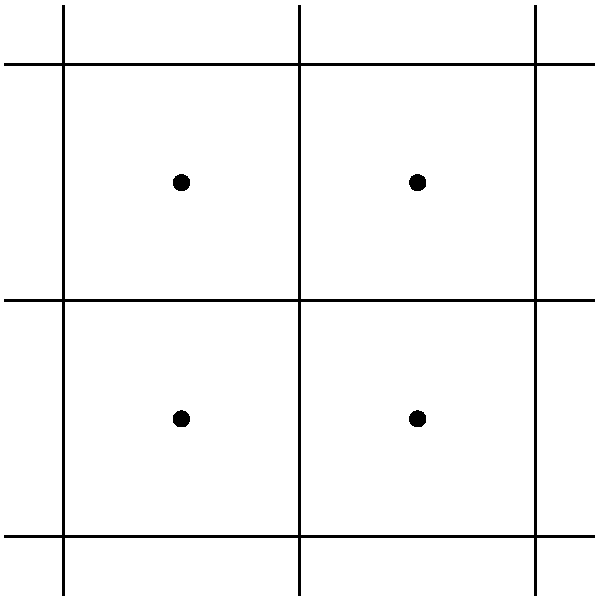
\includegraphics[width=0.4\textwidth]{cellcentred.pdf}
	\caption[Cell-centred grid]{Location of the degrees od freedom in within a 
	cell-centred approach.}
	\label{fig:cellcentred}
\end{figure}

Let us integrate the equation \eqref{eq:cellcentred} over a control volume 
$V_L$ (see Figure~\ref{fig:cctpfa}) and apply the Gauss's divergence theorem:
\begin{equation}
\int_{V_L} \nabla \cdot \mathbf{v} \; dV = \int_{\partial V_L} \mathbf{v} \cdot 
\mathbf{n} \; dA.
\end{equation}
The Forchheimer's law \eqref{eq:forch2} is non-linear, so we use the Newton's 
method in order to compute the velocity, i.e. the flux over the boundary 
$\partial 
V_L$:
\begin{align}
	\mathbf{J}_f(\mathbf{v}^k) \delta \mathbf{v}^{k+1} =& 
	-\mathbf{f}(\mathbf{v}^k), \quad \text{$\forall k\geq 0$ until 
	convergence}\\
	\mathbf{v}^{k+1} =& \mathbf{v}^k + \delta \mathbf{v}^{k+1}
\end{align}
where
\begin{equation} \label{eq:resforch}
	\mathbf{f}(\mathbf{v}) = \mathbf{v} + C_F \sqrt{\mathbf{K}} 
	\frac{\varrho}{\mu} 
	|\mathbf{v}|\mathbf{v} + \frac{1}{\mu} \mathbf{K}(\nabla p - \varrho 
	\mathbf{g} )
\end{equation}
and $\mathbf{J}_f(\mathbf{v})$ is its Jacobian matrix:
\begin{equation} \label{eq:jacforch}
\mathbf{J}_f(\mathbf{v}) = \mathbb{1} + 
C_F\sqrt{\mathbf{K}}\frac{\varrho}{\mu}\big(|\mathbf{v}|\mathbb{1} + 
\frac{1}{|\mathbf{v}|}{\mathbf{v}\mathbf{v}^\mathrm{T}}\big).
\end{equation}
We use as initial guess $\mathbf{v}^0$ the velocity computed with the Darcy's 
law \eqref{eq:darcy}.

The evaluation of \eqref{eq:resforch} and \eqref{eq:jacforch} over $\partial 
V_L$ is performed with a Two Point Flux Approximation (TPFA) method, which 
consists in exploiting the values of the two cells sharing the face; it is a 
simple but robust method, commonly used in commercial software.
\begin{figure}
	\centering
	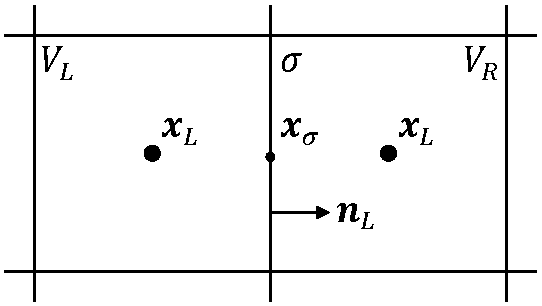
\includegraphics[width=0.6\textwidth]{cctpfa3.pdf}
	\caption{Two cells $V_L$ and $V_R$ sharing the edge $\sigma$.}
	\label{fig:cctpfa}
\end{figure}
Let us consider for instance the face $\sigma = \partial V_L \cup \partial 
V_R$, according to Figure~\ref{fig:cctpfa}, and let the permeability tensor be 
diagonal so that it act as a scalar. We approximate the derivative of the 
pressure $\partial p /\partial 
x$ with a centred finite difference:
\begin{equation}
\frac{\partial p}{\partial x} \simeq \frac{p_R-p_L}{x_R -x_L}.
\end{equation}
We approximate the permeability $\mathbf{K}$ with its value at 
$\mathbf{x}_\sigma$, while 
for the viscosity $\mu$ (and eventually the density $\varrho$) we employ the 
upwind value.

In case of discontinuous permeabilities at the edge $\sigma$, an harmonic 
average weighted on the distances between the cell centres and the edge is 
performed:
\begin{equation}
\frac{|x_R - x_L|}{\mathrm{K}} \simeq 
\frac{|x_\sigma - x_L|}{\mathrm{K}_L}+\frac{|x_R - x_\sigma|}{\mathrm{K}_R}.
\end{equation}

These formulas for the TPFA approximation are the simplified version for a 
Cartesian grid, while in the general case of an unstructured grid the method is 
derived exploiting a decomposition of the vector
\begin{equation}
\mathbf{d}_{L,\sigma}=\mathbf{x}_\sigma - \mathbf{x}_L,
\end{equation}
based the co-normal vector $\mathbf{Kn}_L$ (see \cite{main:tpfa}). Moreover it 
can be shown that this approximation is consistent only if the grid is 
K-orthogonal, i.e. if $\mathbf{Kn}_L$ is parallel to $\mathbf{d}_{L, \sigma}$. 
%\section{Coupling conditions}
% Disegno di cosa succede all'interfaccia
% Not sure about this section...
\section{Time discretization}
For the temporal discretization we employ fully implicit, unconditionally 
stable methods as the Backward Euler (BE) and the Backward Differencing Formula 
2 (BDF2) also for non constant time steps. A monolithic approach is used, the 
Jacobian matrix is computed 
numerically then the UMFPACK solver is used. The time-step size depends of the 
convergence of the Newton's method at the previous time iteration.
\section{Summary}
Fully implicit coupling, monolithic approach, UMFPACK, cenni alle coupling 
conditions and boundary conditions, primary variables.